\icode{N24W-MM-CA-L3-260625-001}
\nceeID{2024安徽}{14}
如图所示，一实验小车静止在光滑水平面上，其上表面有粗糙水平轨道与光滑四分之一圆弧轨道。圆弧轨道与水平轨道相切于圆弧轨道最低点，一物块静止于小车最左端，一小球用不可伸长的轻质细线悬挂于\(O\)点正下方，并轻靠在物块右侧。现将细线拉直到水平位置时，静止释放小球，小球运动到最低点时与物块发生弹性碰撞。碰撞后，物块沿着的轨道运动，已知细线长\(L =\)\,\qty{1.25}{m}。小球质量\(m =\)\,\qty{0.20}{kg}。物块、小车质量均为\(M =\)\,\qty{0.30}{kg}。小车上的水平轨道长\(s =\)\,\qty{1.0}{m}。圆弧轨道半径\(R =\)\,\qty{0.15}{m}。小球、物块均可视为质点。不计空气阻力，重力加速度\(g\)取\,\qty{10}{m/s^2}。
\begin{enumerate}
	\item[(1)] 求小球运动到最低点与物块碰撞前所受拉力的大小；
	\item[(2)] 求小球与物块碰撞后的瞬间，物块速度的大小；
	\item[(3)] 为使物块能进入圆弧轨道，且在上升阶段不脱离小车，求物块与水平轨道间 动摩擦因数 的取值范围。
\end{enumerate}

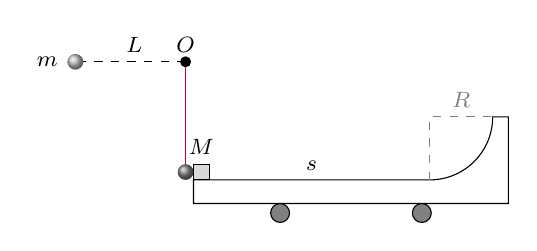
\begin{tikzpicture}
	\draw (0,0.3)--node[above]{\footnotesize\(s\)}(3,.3) arc(-90:0:.8)--(4,1.1)--(4,0)--(0,0)--(0,.3);
	\draw[fill=gray] (1.1,-.12) circle(.12) (2.9,-.12) circle(.12);
	\draw[gray,dashed] (3,.3)--(3,1.1)--node[above]{\footnotesize\(R\)}(3.8,1.1);
	\draw[fill=gray!30] (0,.3) rectangle(.2,.5);
	\shade[ball color=gray] (-.1,.4) circle(.1);
	\draw[purple](-.1,.5)--(-.1,1.8)node[above,black]{\footnotesize\(O\)};
	\draw[dashed] (-.1,1.8)--node[above]{\footnotesize\(L\)}(-1.4,1.8);
	\shade[ball color=gray!50] (-1.5,1.8) circle(.1);
	\node at(-1.6,1.8)[left]{\footnotesize\(m\)};
	\node at(.1,.5)[above]{\footnotesize\(M\)};
	\fill (-.1,1.8) circle(.07);
\end{tikzpicture}